\documentclass[tikz,border=2pt,11pt]{standalone}
\usetikzlibrary{arrows.meta}
\usetikzlibrary{decorations.pathreplacing}
\usetikzlibrary{calc}
\usetikzlibrary{patterns}
\usetikzlibrary{positioning}
\usepackage{amsmath}
\usepackage{amssymb}
\usepackage{bm}
\usepackage{graphicx}
\usepackage{xcolor}
\usepackage{tikz}
\newcommand{\R}{\mathbb R}
\newcommand{\C}{\mathbb C}
\newcommand{\Z}{\mathbb Z}
\newcommand{\N}{\mathbb N}
\newcommand{\Q}{\mathbb Q}
\newcommand{\E}{\mathbb E}
\newcommand{\Prob}{\mathbb P}
\newcommand{\widehatC}{\widehat{\mathbb C}}
\newcommand{\eps}{\varepsilon}
\newcommand{\dd}{\,\mathrm d}
\newcommand{\ind}{\mathbf 1}
\newcommand{\one}{\mathbf 1}
\newcommand{\law}{\operatorname{Law}}
\newcommand{\supp}{\operatorname{supp}}
\newcommand{\diam}{\operatorname{diam}}
\newcommand{\dist}{\operatorname{dist}}
\newcommand{\Leb}{\operatorname{Leb}}
\newcommand{\Var}{\operatorname{Var}}
\newcommand{\Cov}{\operatorname{Cov}}
\newcommand{\id}{\operatorname{id}}
\newcommand{\sgn}{\operatorname{sgn}}
\newcommand{\rank}{\operatorname{rank}}
\newcommand{\tr}{\operatorname{tr}}
\newcommand{\EL}{\operatorname{EL}}
\newcommand{\CLE}{\mathrm{CLE}}
\newcommand{\SLE}{\mathrm{SLE}}
\newcommand{\LQG}{\mathrm{LQG}}
\newcommand{\GFF}{\mathrm{GFF}}
\newcommand{\FK}{\mathrm{FK}}
\newcommand{\PV}{\operatorname{PV}}
\newcommand{\cB}{\mathcal B}
\newcommand{\cF}{\mathcal F}
\newcommand{\cG}{\mathcal G}
\newcommand{\cK}{\mathcal K}
\newcommand{\cT}{\mathcal T}
\newcommand{\cU}{\mathcal U}
\newcommand{\cV}{\mathcal V}
\newcommand{\cW}{\mathcal W}
\newcommand{\cL}{\mathcal L}
\newcommand{\cH}{\mathcal H}
\newcommand{\cA}{\mathcal A}
\newcommand{\cD}{\mathcal D}
\newcommand{\cM}{\mathcal M}
\newcommand{\cP}{\mathcal P}
\newcommand{\cS}{\mathcal S}
\newcommand{\cI}{\mathcal I}
\newcommand{\cJ}{\mathcal J}
\newcommand{\proofstage}[1]{\par\Needspace{4\baselineskip}\smallskip
  \noindent\textit{#1.}\par\nopagebreak\smallskip\nopagebreak}
\begin{document}
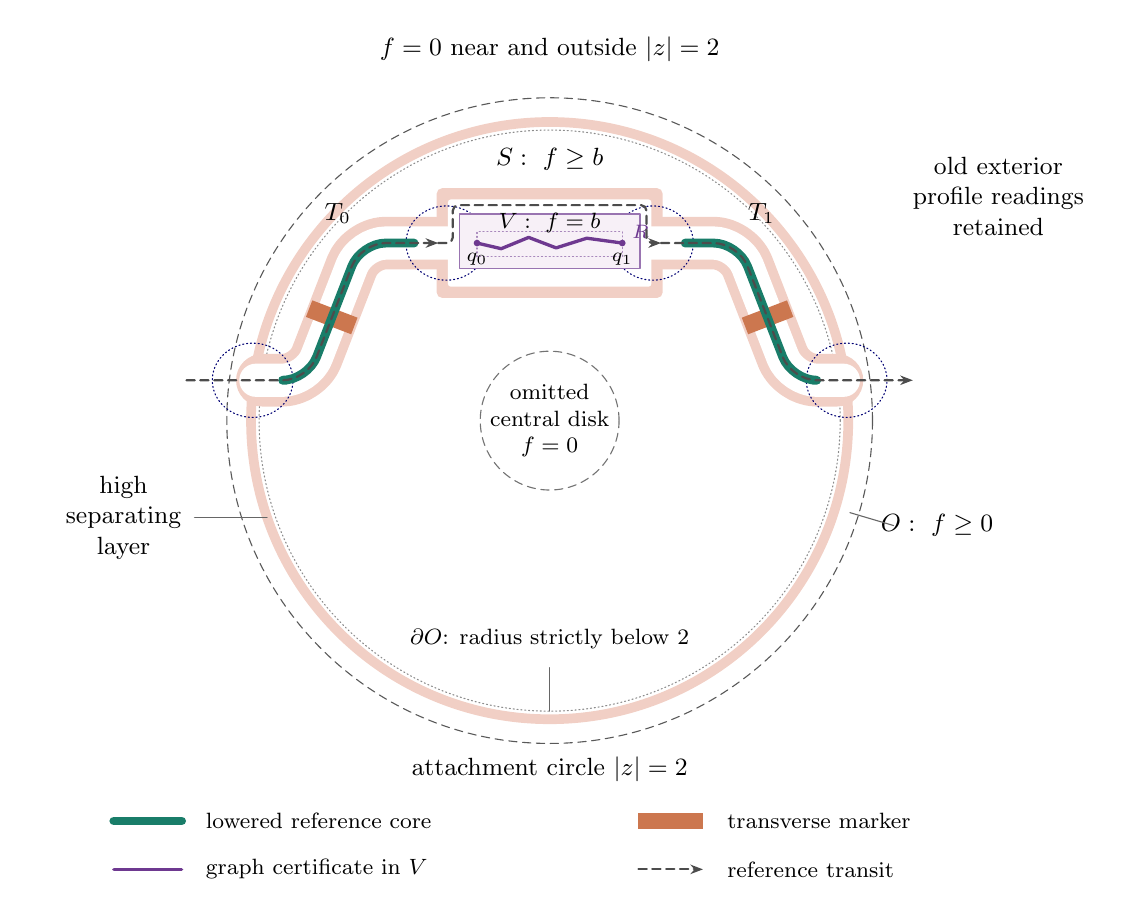
\begin{tikzpicture}[x=2.05cm,y=2.05cm,font=\small,
  line cap=round,line join=round,
  guide/.style={black!60,thin},
  refpath/.style={black!70,densely dashed,thick,
    -{Stealth[length=1.6mm]}},
  shortcutcap/.style={draw=blue!45!black,densely dotted,thin},
  note/.style={align=center,font=\small}]
\definecolor{shortcutwall}{RGB}{241,207,197}
\definecolor{shortcutmarker}{RGB}{204,119,79}
\definecolor{shortcutcore}{RGB}{25,125,105}
\definecolor{shortcutcert}{RGB}{110,57,144}

\draw[black!65,densely dashed] (0,0) circle (2);
\draw[black!45,densely dotted] (0,0) circle (1.80);

\fill[shortcutwall,even odd rule]
  (0,0) circle (1.88) (0,0) circle (1.82);
\draw[shortcutwall,line width=19pt,rounded corners=9pt]
  (-1.78,.25) -- (-1.50,.25) -- (-1.17,1.10) -- (-.57,1.10);
\draw[shortcutwall,line width=19pt,rounded corners=9pt]
  (1.78,.25) -- (1.50,.25) -- (1.17,1.10) -- (.57,1.10);
\fill[shortcutwall,rounded corners=2pt]
  (-.70,.76) rectangle (.70,1.44);
\draw[white,line width=12pt,rounded corners=9pt]
  (-1.82,.25) -- (-1.50,.25) -- (-1.17,1.10) -- (-.57,1.10);
\draw[white,line width=12pt,rounded corners=9pt]
  (1.82,.25) -- (1.50,.25) -- (1.17,1.10) -- (.57,1.10);
\fill[white,rounded corners=1pt]
  (-.63,.83) rectangle (.63,1.37);

\fill[white] (0,0) circle (.43);
\draw[black!55,densely dashed] (0,0) circle (.43);
\node[note,font=\footnotesize] at (0,0)
  {omitted\\central disk\\$f=0$};

\draw[shortcutcap] (-1.84,.25) ellipse [x radius=.25,y radius=.23];
\draw[shortcutcap] (1.84,.25) ellipse [x radius=.25,y radius=.23];
\draw[shortcutcap] (-.64,1.10) ellipse [x radius=.25,y radius=.23];
\draw[shortcutcap] (.64,1.10) ellipse [x radius=.25,y radius=.23];

\begin{scope}[shift={(-1.35,.64)},rotate=69]
  \fill[shortcutmarker] (-.055,-.15) rectangle (.055,.15);
\end{scope}
\begin{scope}[shift={(1.35,.64)},rotate=-69]
  \fill[shortcutmarker] (-.055,-.15) rectangle (.055,.15);
\end{scope}

\draw[shortcutcore,line width=3.2pt,rounded corners=9pt]
  (-1.63,.25) -- (-1.50,.25) -- (-1.17,1.10) -- (-.84,1.10);
\draw[shortcutcore,line width=3.2pt,rounded corners=9pt]
  (1.63,.25) -- (1.50,.25) -- (1.17,1.10) -- (.84,1.10);

\filldraw[fill=violet!6,draw=shortcutcert!70,thin]
  (-.56,.94) rectangle (.56,1.28);
\draw[shortcutcert!60,densely dotted,thin]
  (-.45,1.015) rectangle (.45,1.17);
\node[font=\footnotesize] at (0,1.225) {$V:\ f=b$};
\draw[shortcutcert,very thick]
  (-.45,1.10) -- (-.30,1.065) -- (-.13,1.135)
  -- (.04,1.07) -- (.23,1.13) -- (.45,1.10);
\fill[shortcutcert] (-.45,1.10) circle (1.2pt);
\fill[shortcutcert] (.45,1.10) circle (1.2pt);
\node[below,font=\scriptsize] at (-.45,1.095) {$q_0$};
\node[below,font=\scriptsize] at (.45,1.095) {$q_1$};
\node[right,font=\scriptsize,text=shortcutcert] at (.45,1.17) {$R$};

\draw[refpath,rounded corners=9pt]
  (-2.25,.25) -- (-1.50,.25) -- (-1.17,1.10) -- (-.69,1.10);
\draw[refpath,rounded corners=2pt]
  (-.69,1.10) -- (-.60,1.10) -- (-.60,1.335)
  -- (.60,1.335) -- (.60,1.10) -- (.69,1.10);
\draw[refpath,rounded corners=9pt]
  (.69,1.10) -- (1.17,1.10) -- (1.50,.25) -- (2.25,.25);

\node[above] at (0,1.49) {$S:\ f\ge b$};
\node[above left] at (-1.17,1.16) {$T_0$};
\node[above right] at (1.17,1.16) {$T_1$};
\node[note] at (0,2.30) {$f=0$ near and outside $|z|=2$};
\node[note,text width=2.7cm] at (2.78,1.39)
  {old exterior\\profile readings\\retained};
\node[note] at (2.40,-.65) {$O:\ f\ge0$};
\draw[guide] (2.13,-.65) -- (1.86,-.57);
\node[note,text width=2.2cm] at (-2.64,-.60)
  {high\\separating\\layer};
\draw[guide] (-2.20,-.60) -- (-1.75,-.60);
\node[below] at (0,-2.02) {attachment circle $|z|=2$};
\node[note,font=\footnotesize] at (0,-1.35)
  {$\partial O$: radius strictly below $2$};
\draw[guide] (0,-1.53) -- (0,-1.80);

\draw[shortcutcore,line width=3.2pt] (-2.70,-2.48) -- (-2.28,-2.48);
\node[right,font=\footnotesize] at (-2.19,-2.48) {lowered reference core};
\fill[shortcutmarker] (.55,-2.53) rectangle (.95,-2.43);
\node[right,font=\footnotesize] at (1.04,-2.48) {transverse marker};
\draw[shortcutcert,very thick] (-2.70,-2.78) -- (-2.28,-2.78);
\node[right,font=\footnotesize] at (-2.19,-2.78) {graph certificate in $V$};
\draw[refpath] (.55,-2.78) -- (.95,-2.78);
\node[right,font=\footnotesize] at (1.04,-2.78) {reference transit};
\end{tikzpicture}
\end{document}
